\documentclass[12pt]{report} %fuente a 12pt

% MÁRGENES: 2,5 cm sup. e inf.; 3 cm izdo. y dcho.
\usepackage[
a4paper,
vmargin=2.5cm,
hmargin=3cm
]{geometry}

% ENLACES
\usepackage{hyperref}
\hypersetup{colorlinks=true,
	linkcolor=black, % enlaces a partes del documento (p.e. índice) en color negro
    urlcolor=blue} % enlaces a recursos fuera del documento en azul
    
\usepackage[spanish, es-tabla]{babel}
\usepackage{graphicx}
\usepackage{float}
\usepackage{listings}
\usepackage[titletoc,toc,page]{appendix}
\renewcommand{\appendixtocname}{Ap\'endices}
\renewcommand{\appendixpagename}{Ap\'endices}

% REVISAR FUENTES
% REVISAR FOTOS
% REVISAR NEGRITAS
% REVISAR CURSIVA

\title{Lyncex: describiendo una aplicación web como conocimiento}
\author{Adrián Arroyo Calle}
\date{Curso 2019-2020}

\begin{document}

\maketitle

\tableofcontents

\listoffigures

\listoftables

\chapter{Introducción}

\section{Motivación}

En ciencias de la computación, de forma recurrente se divide entre código, lo que va a ejecutar la máquina, y datos.
Esta diferencia, aunque pueda resultar evidente, es innecesaria, ya que el código no deja de ser dato, solo que con una semántica diferente.
Von Neuman, en su modelo de computadora, elimina las diferencias a nivel de hardware entre código y datos, de modo muy exitoso, hasta tal punto que esta idea sigue siendo la base de los procesadores modernos actuales.
Hoy día en la creación de aplicaciones web, separamos por un lado el código y por otro los datos que van a circular a través de él. 
No obstante, considero interesante imaginar y plantear una aplicación web descrita de la misma forma en que se describen los datos.
De forma principalmente declarativa y usando tecnologías maduras como RDF como la base del modelo de datos.
El servidor web pasa a ser una base de datos, dónde las diferencias entre código y datos son puramente semánticas.

De este modo, podríamos resumir este sistema como una base de datos y a la vez un servidor web configurable a través del contenido semántico de la propia base de datos.

La idea surge principalmente de estudiar la base de datos CouchDB (se detallará más adelante) y su concepto de integrar código JavaScript como un tipo de documento más.

\section{Objetivos}

El objetivo principal de este trabajo es construir una entorno de desarrollo que implemente el concepto de base de datos y servidor web en un mismo entorno, usando tripletas para su representación. Sobre esta plataforma deberán poder ejecutarse aplicaciones simples y la llamaremos a partir de ahora, Lyncex.

La implementación resultante no deberá ser de un nivel de producción, pero deberá ser útil para validar los conceptos con los que se va a trabajar, así como el estado de ciertas tecnologías con de relativa poca popularidad en el mundo empresarial.

Además de la implementación en código, se definirá una ontología que define el funcionamiento de la aplicación web. Esta ontología es una interfaz sobre la que un trabajo posterior podría diseñar implementaciones alternativas, mejorando el código original o extendiendo la funcionalidad.

En este proyecto se reforzarán los conocimientos del lenguaje Prolog, en concreto en una vertiente altamente práctica, como es su utilidad para desarrollo de aplicaciones web.

\section{Alcance}

\section{Aplicación de ejemplo (visión general)}

De nada serviría una plataforma de desarrollo completa sin aplicaciones que la utilicen. Para demostrar la funcionalidad del sistema, en entornos reales, se diseñará una aplicación basada en datos abiertos ya existentes.

Se usarán los datos de Bibliotecas de Castilla y León, en formato RDF/XML y se tratará de hacer un ejemplo práctico de aplicación modelo que usa Lyncex.

\section{Estructura de la memoria}
La memoria se estructura en diferentes capítulos. En primer lugar, se repasarán conocimientos previos necesarios para entender, desde una base técnica pero no especializada, el conjunto de este trabajo. Posteriormente se realizará el análisis de diferentes tecnologías similares, que cubren parte de los objetivos de este trabajo de alguna u otra forma, el conocido como estado del arte.

Posteriormente se tratará la planificación del proyecto, haciendo un inciso en la metodología SCRUM. Posteriormente se pasará a la etapa de análisis, donde se descompondrán los requisitos del proyecto y las historias de usuario a realizar.

El siguiente capítulo está dedicado al diseño, tanto del propio software, como de la ontología que lo acompaña. A continuación, se encuentra el capítulo de la implementación. En este capítulo primero veremos herramientas que se han usado para la construcción de este proyecto. Después veremos la implementación del software en sí, haciendo especial hincapié en aquellos elementos que no sean del todo evidentes para el lector.

El capítulo dedicado a la validación y las pruebas se ubica inmediatamente después. En este capítulo se describirán las pruebas realizadas y la metodología empleada para comprobar que efectivamente, se está implementando correctamente el software.

Le sigue el capítulo dedicado a la aplicación de ejemplo, donde se llevará a cabo un mini proyecto (objetivo, análisis, diseño, implementación y pruebas) para ver que el software como plataforma de desarrollo para otras aplicaciones tiene sentido o no, y poder identificar posibles inconvenientes prácticos que se hayan encontrado.

A modo de referencia, el capítulo de manuales, incluye instrucciones de instalación y de uso de Lyncex.

Por último, se hablará sobre las conclusiones que podemos extraer del proyecto así como trabajo que podría realizarse en el futuro siguiendo por este camino.


\chapter{Conocimientos previos}

En este capítulo trataremos de explicar de la forma más clara posible, conocimientos que creemos necesarios para entender el proyecto en su totalidad.

\section{Web Semántica}

La web semántica es un concepto amplio, surgido a finales de los 90 y en un principio impulsado por Tim Berners-Lee y su organización, el W3C. La idea principal es dar un paso cualtitativo más en el acceso y descripción de datos respecto al modelo de la web HTML. Dentro de este paraguas existen numerosos proyectos como RDF, SPARQL, LinkedData, ... En este proyecto solo utilizamos algunas de ellas.

\subsection{RDF}

RDF es una de las tecnologías base, sobre las que se asienta prácticamente toda la web semántica. Se trata de un modelo de representación de la información basado en tripletas.

\subsubsection{Tripletas}
Las tripletas son un modo de representar la información mediante tríos, ordenados, de datos.
Es uno de los modos fundamentales de representación de información

En una tripleta, los elementos se denominan, en este orden, sujeto, predicado y objeto. La estructura básica sigue la de la gramática del lenguaje humano para afirmar hechos.
El sujeto es el ente sobre el que vamos a afirmar algo, el predicado es la acción y/o propiedad del sujeto y el objeto, que es el contenido de la propiedad que se define.
Veamos algunos ejemplos de este concepto:
\begin{verbatim}
maria -> likes -> chocolate
maria -> is -> human
adrian -> likes -> maria
\end{verbatim}
Con estos tres elementos, y suponiendo que podemos combinar sujetos, predicados y objetos en otras tripletas, podemos crear grandes redes interrelacionadas, ideales para el almacenamiento de conocimiento.
Estas se denominan grafos.
Tres es el número mínimo necesario para poder modelar cualquier descriptible. Las duplas (dos elementos) también son populares en bases de datos, pero necesitan de un contexto externo para su interpretación correcta.
Este sistema además tiene varias ventajas, por ejemplo, la duplicación de las tripletas no es un problema, ya que simplemente se reafirma lo mismo una y otra vez.

La idea de las tripletas es bastante genérica y existen diferentes implementaciones de la idea. La más popular, sin lugar a dudas, es RDF, que describiremos a continuación.
Las tripletas tienen numerosas ventajas pero también diversos inconvenientes, entre ellos: rendimiento inferior y mayor dificultad a la hora de actualizar el contenido de las tripletas.
Esto, sumado a la falta de educación en este concepto, ha provocado que actualmente, el uso de tripletas sea minoritario.

\subsubsection{Tripletas en RDF}

RDF (Resource Description Framework) es un estándar desarrollado por Tim Berners-Lee en los años 90.
RDF define un modelo concreto para usar tripletas derivado de la World Wide Web, para ello se impone que los elementos o términos puedan ser solo de tres tipos: IRIs, blank nodes y literales.
Las IRIs son la versión internacionalizada y ampliada de las famosas URL. Cada IRI representa un recurso, tratándose de un identificadores universal y son la base de las interconexiones entre tripletas. En RDF se pueden usar IRIs en el sujeto, el predicado y el objeto.
Los literales son datos puros, sin conexión entre sí. Pueden ser cadenas de texto, números enteros, números decimales, etc... Solo los objetos pueden ser literales.
Los blank nodes son conexiones anónimas, sin definir explícitamente, entre varias tripletas. Solo pueden ser blank nodes los sujetos y los objetos.

Además RDF define ciertos recursos de utilidad como un tipado y una distinción entre varios tipos elementales de recurso.

RDF se define sin representación textual por defecto, aunque existen varios estándares. Uno de los originales es RDF-XML, que usa la sintaxis de XML para definir RDF. Esta sintaxis es especialmente compleja, ya que es verbosa y admite varios modos de uso.
Otros estándares definen JSON-LD que usa sintaxis de JSON, otro formato genérico popular o RDFa que se integra en HTML. Sin embargo, también existen sintaxis expresamente diseñadas para RDF, que por lo general son más claras que tratar de adaptar otro formato a RDF.
Algunos ejemplos de estas sintaxis son Turtle, N3, NTriples y TriG.

En Lyncex se ha decidido usar sintaxis Turtle. Un ejemplo de esta sintaxis a continuación:

\begin{lstlisting}
@base <https://lyncex.com/lyncex#> .
@prefix rdf: <http://www.w3.org/1999/02/22-rdf-syntax-ns#> .
@prefix foaf: <http://xmlns.com/foaf/0.1/> .

<Richard_Feynman>
    a foaf:Person ;
    foaf:name "Richard Feynman" ;
    foaf:birthday "02-15" ;
    foaf:knows [
        a foaf:Person ;
        foaf:name "Albert Einstein"
    ] ;
    foaf:knows <Von_Neumman> .

<Von_Neumman>
    a foaf:Person ;
    foaf:name "John Von Neumman" .
\end{lstlisting}

Que es equivalente a:
\begin{verbatim}
https://lyncex.com/lyncex#Richard_Feynman -> http://www.w3.org/1999/02/22-rdf-syntax-ns#type -> http://xmlns.com/foaf/0.1/Person
https://lyncex.com/lyncex#Richard_Feynman -> http://xmlns.com/foaf/0.1/name -> Richard Feynman
https://lyncex.com/lyncex#Richard_Feynman -> http://xmlns.com/foaf/0.1/birthday -> "02-15"
https://lyncex.com/lyncex#Richard_Feynman -> http://xmlns.com/foaf/0.1/knows -> _:1
https://lyncex.com/lyncex#Richard_Feynman -> http://xmlns.com/foaf/0.1/knows -> https://lyncex.com/lyncex#Von_Neumman
_:1 -> http://www.w3.org/1999/02/22-rdf-syntax-ns#type -> http://xmlns.com/foaf/0.1/Person
_:1 -> http://xmlns.com/foaf/0.1/name -> Albert Einstein
https://lyncex.com/lyncex#Von_Neumman -> http://www.w3.org/1999/02/22-rdf-syntax-ns#type -> http://xmlns.com/foaf/0.1/Person
https://lyncex.com/lyncex#Von_Neumman -> http://xmlns.com/foaf/0.1/name -> John Von Neumman
\end{verbatim}

En Turtle primero se inicia definiendo una base para las IRIs y prefijos para no tener que escribir IRIs largas y poco legibles en el resto del documento.
Las IRIs se definen usando los símbolos < y >. Las IRIs con prefijo llevan el prefijo y el símbolo :. 
Los literales llevan comillas y los blank nodes se definen con [ y ] y en su interior se definen las tripletas teniendo como sujeto el propio blank node.

En Turtle existe una forma sencilla de no repetir el sujeto, útil para afirmar varias cosas sobre un mismo sujeto. Se utiliza el símbolo ; para iniciar una nueva tripleta sobre el mismo sujeto.

Al acabar de afirmar cosas sobre un sujeto, se pone un punto. Un azúcar sintáctico usado en el ejemplo es que la propiedad a es equivalente a \begin{verbatim}http://www.w3.org/1999/02/22-rdf-syntax-ns#type\end{verbatim}.

\subsection{RDF schema y ontologías}

RDF es un modelo de representación de la información muy potente, sin embargo, tal y como lo hemos definido, puede volverse muy caótico en poco tiempo.

La razón es que no hay ningún requisito per sé de como tienen que estructurarse los datos dentro de las tripletas. El principal inconveniente de esto es la interoperabilidad entre diferentes fuentes de información y entre diferentes programas.

Para solucionarlo, una idea que se puede tener es disponer de unos metadatos que informen de como se debe manejar esta información. Esta información que describe la estructura de otra información se denomina ontología. Ya que las ontologías no son más que información, se incorpora como tripletas también y no existe diferencia física de entre las tripletas de una ontología y la de una información cualquiera, la diferencia es puramente semántica. 

Existen numerosos lenguajes de ontologías bajo RDF, uno de los primeros, impulsado como estándar por el W3C es RDF Schema. Existen otros lenguajes más avanzados como OWL, que incluyen soporte para descripciones más elaboradas.

La base de RDF Schema es la clase, o rdfs:Class, usando la IRI con prefijos. Las clases a su vez pueden ser subclases de otra con rdfs:subClassOf. Las clases podemos usarlas para definir tipos nuevos, que luego se referencian usando la propiedad rdf:type.

A su vez, también podemos definir los predicados, también llamados propiedades. Esto ya venía en RDF, bajo el tipo rdf:Property, pero RDF Schema añade predicados extras como rdfs:domain y rdfs:range. El primero permite definir en una tripleta que usa esta propiedad los elementos de que tipo pueden ser sujetos. Y en el caso del range que clase de valores de aceptan como objeto. Las propiedades se pueden heredar también mediante rdfs:subPropertyOf.

Con estos elementos podemos crear ontologías con esquemas similares a los que tendríamos en programación orientada a objetos, aunque de forma mucho más flexible.

\subsection{SPARQL}

\section{Prolog}

\chapter{Estado del Arte}

Antes de adentrarnos en los detalles de Lyncex conviene recapitular ideas similares ya existentes así como herramientas que nos puedan ayudar. 

\section{Frameworks web}

\subsection{Django}
Django es uno de los frameworks web más populares dentro del mundo Python y es una referencia dentro del mundo de los frameworks web por su potencia y claridad de código.\cite{django}
Fuertemente inspirado por \textbf{Ruby on Rails}, adopta de él su filosofía DRY (Don't Repeat Yourself) y su \textit{convention over configuration}.
El framework trabaja con bases de datos relacionales principalmente, pero es una buena base para diseñar la semántica del servidor web.

Django sigue una arquitctura MTV, es decir, Model-Template-View. Es bastante similar al popular MVC, aunque según sus creadores, el controlador es el propio framework.
En Django el modelo se define como una clase de Python, que gracias al ORM, tiene persistencia en la base de datos. La parte de las plantillas se programa con un lenguaje similar a HTML, pero con capacidad de mostrar variables
y de cierta lógica (condicional, bucle) con metaetiquetas. La parte de vista es código Python puro. Existe un fichero especial llamado urls.py que contiene un listado que relaciona las URLs con las vistas.

Las vistas pueden acceder a los parámetros GET o POST directamente y operar sobre ellos así como a la sesión del usuario que visita la página.
Las vistas en Django pueden protegerse mediante un sistema de autenticación sencillo pero seguro, que permite bloquear fácilmente o redirigir si el usuario no ha iniciado sesión o si no tiene los permisos suficientes.
Estas características de Django tienen el denominador común de que son implementadas usando middleware, es decir, componentes del framework que se introducen entre la petición bruta original
y la vista.

Otra característica interesante de Django apoyada en el middleware es la gestión de formularios. Los formularios se definen en Django como una clase más, parecida a un modelo de base de datos (de hecho, se puede hacer que sea la misma clase).
Con esta clase Django puede generar parte de la plantilla automáticamente. Posteriormente, en el método POST, el middleware puede limpiar y validar los campos, de modo que a la vista llegan ya los datos limpios.

Por último, existe un componente llamado \textbf{Django REST Framework}, que añade funcionalidad para diseñar una API REST con los mismos patrones y facilidades que el desarrollo web HTML.

\section{Bases de datos}
\subsection{Apache CouchDB}
Apache CouchDB es una base de datos NoSQL de tipo documental, almacenados estos en formato JSON.\cite{couchdb}
Su peculiaridad respecto a otras bases de datos similares como MongoDB viene por la forma de acceder a los datos.
Aunque en las últimas versiones CouchDB también dispone de un lenguaje de consulta, la forma original de acceder a la información era programando lo que se denominan vistas, en JavaScript.
Estas vistas generan un endpoint HTTP, que al ser llamado ejecutan el código JavaScript, en dos pasos. Primero un paso de map, para seleccionar los datos y realizar alguna transformación individual.
Posteriormente un paso de reduce permite realizar agregaciones. El código JavaScript que se ejecuta se almacena en la base de datos junto al resto de documentos.

Para interactuar con la base de datos se dispone de una API HTTP, tanto para crear como para borrar y o modificar los documentos.
Además dispone de un sistema de replicación entre nodos eventualmente consistente y relativamente simple, de forma que hay otros proyectos que implementan el mismo protocolo (PouchDB para navegadores web por ejemplo).

\subsection{TerminusDB}
TerminusDB es una base de datos programada en Prolog que comparte junto a CouchDB la característica de ser de tipo NoSQL de tipo documental.\cite{terminusdb}
Sin embargo, TerminusDB almacena tripletas RDF. RDF, como veremos más adelante, es un modelo de representación del conocimiento basado en tripletas.
TerminusDB cuenta con un lenguaje de consulta propio, admite ciertas validaciones sobre los datos y también dispone de una API HTTP.
TerminusDB no dispone de ninguna característica similar a las vistas de CouchDB.

\section{Triplestores}

\subsection{Apache Jena}
Apache Jena es una base de datos de tripletas RDF, una de las más maduras si nos atenemos a su longevidad (Jena 1.0 es del año 2000).\cite{couchdb}
Implementa gran cantidad de estándares de la web semántica como RDF, RDF Schema, SPARQL, OWL, etc sin embargo no dispone tampoco de la capacidad de generar vistas web.

\subsection{Virtuoso y Marklogic}
OpenLink Virtuoso y MarkLogic son bases de datos multimodelo, entre ellos soportan el almacenamiento de tripletas.\cite{virtuoso}\cite{marklogic}.
Virtuoso tiene una versión opensource usada detrás de grandes silos de conocimiento como DBPedia o Wikidata. Ambas soportan queries vía SPARQL.

\subsection{ClioPatria}
ClioPatria es una aplicación que combina las librerías de RDF y HTTP de SWI-Prolog para ofrecer una base de datos semántica completa.\cite{cliopatria}
Soporta queries en SPARQL, SeRQL y en código Prolog. Al estar basada la aplicación en componentes independientes, podemos usarlos como base
de nuestra aplicación.

\section{Análisis}

Esta tabla representa como cumplen los objetivos propuestos en la sección Objetivos en cada uno de los programas analizados.


\begin{table}[ht]
    \resizebox{\textwidth}{!}{%
    \begin{tabular}{llllllll}
                  & \textbf{CouchDB} & \textbf{TerminusDB} & \textbf{Django} & \textbf{Jena} & \textbf{Virtuoso} & \textbf{ClioPatria} & \textbf{Lyncex} \\
    \textbf{Almacén tripletas}  & No               & Sí                  & Sí (1)          & Sí            & Sí            & Sí                  & Sí              \\
    \textbf{Ontología disponible}  & No               & No                  & No              & No            & No                & No                  & Sí              \\
    \textbf{Webs estáticas}  & Sí               & No                  & Sí              & No            & No                & No                  & Sí              \\
    \textbf{Webs plantillas}  & Sí               & No                  & Sí              & No            & No                & No                  & Sí              \\
    \textbf{Webs CRUD}  & Sí               & No                  & Sí              & No            & No                & No                  & Sí              \\
    \textbf{Autenticación} & Sí               & No                  & Sí              & No            & No                & No                  & No              \\
    \textbf{APIs} & Sí               & No                  & Sí (2)          & No            & No                & No                  & No              \\
    \textbf{SPARQL} & No               & No                  & No              & Sí            & Sí                & Sí                  & No             
    \end{tabular}
    }
\end{table}

Notas:
\begin{enumerate}
    \item Aunque Django cuenta con un ORM muy potente para trabajar sobre el modelo relacional, nada impide usar otros modelos de almacenamiento.
    \item A través de Django REST Framework, un componente independiente pero altamente acoplado
\end{enumerate}

\chapter{Planificación}

\section{SCRUM}
\subsection{Introducción}
\subsection{Actores}
\subsection{Eventos}
\subsection{Artefactos}
\section{Metodología de trabajo}
\section{Plan de gestión de riesgos}
\section{Suposiciones y restricciones}
Para el proyecto se ha tratado de seguir una metodología similar a SCRUM, obviando ciertas diferencias inherentes al trabajo invididual.
Primero se realizó una estimación, basada en puntos de historia, de cada una de las historias de usuario, pasando a formar parte del product backlog.
Estas historias de usuario representan los 5 objetivos mencionados anteriormente y existen ciertas dependencias entre ellas tal y como se puede ver en el gráfico.

\begin{figure}[h]
    \centering
    \includegraphics[width=\textwidth]{plantuml/dependency.png}
    \caption{Dependencias entre las historias de usuario}
    \label{fig:dependencia}
\end{figure}

Merece especial mención la historia de usuario de desarrollo de ontología. Si bien podría ser un requisito previo de cara a otras historias de usuario, en la práctica
se han desarrollado de forma paralela, añadiendo lo necesario a la ontología en cada historia de usuario nueva.

Cada una de estas historias de usuario tenía asociadas diferentes condiciones de aceptación. Se trata de frases que siguen el estilo: Dado/Cuando/Entonces. 
Una implementación completa de la historia de usuario hará que todas las frases sean ciertas. Gracias a Behave, estas condiciones de aceptación no solo existen en el papel, sino en el código también que comprueba de forma activa además que no haya regresiones en etapas posteriores.

Estas historias de usuario a su vez se descompusieron en tareas lo más atómicas posibles, normalmente con una condición de aceptación asociada para saber que la tarea había acabado.

En metodología SCRUM, el trabajo se divide en sprints de varias semanas. En este caso en particular se eligieron sprints de tres semanas, aunque el tiempo real se decidía al inicio del sprint.
En esta reunión se elegían las tareas que debían a formar parte del sprint, formando parte de una lista conocida como sprint backlog.

En nuestra implementación particular de SCRUM, no había equipo, por tanto ciertos roles y ceremonias dejaban de tener interés. 
En este sentido, no se realizaron dailies y tanto el Product Owner como el equipo de desarrollo recayeron en mi persona, pudiendo asimilar el rol de Scrum Master al tutor del proyecto, Miguel Ángel Martínez Prieto.

\chapter{Análisis y diseño}

\section{Requisitos}

\section{Diseño de Lyncex}

\subsection{Arquitectura}

\subsection{API}

\subsection{Controladores}

\section{Diseño de la ontología}

\begin{figure}[h]
    \centering
    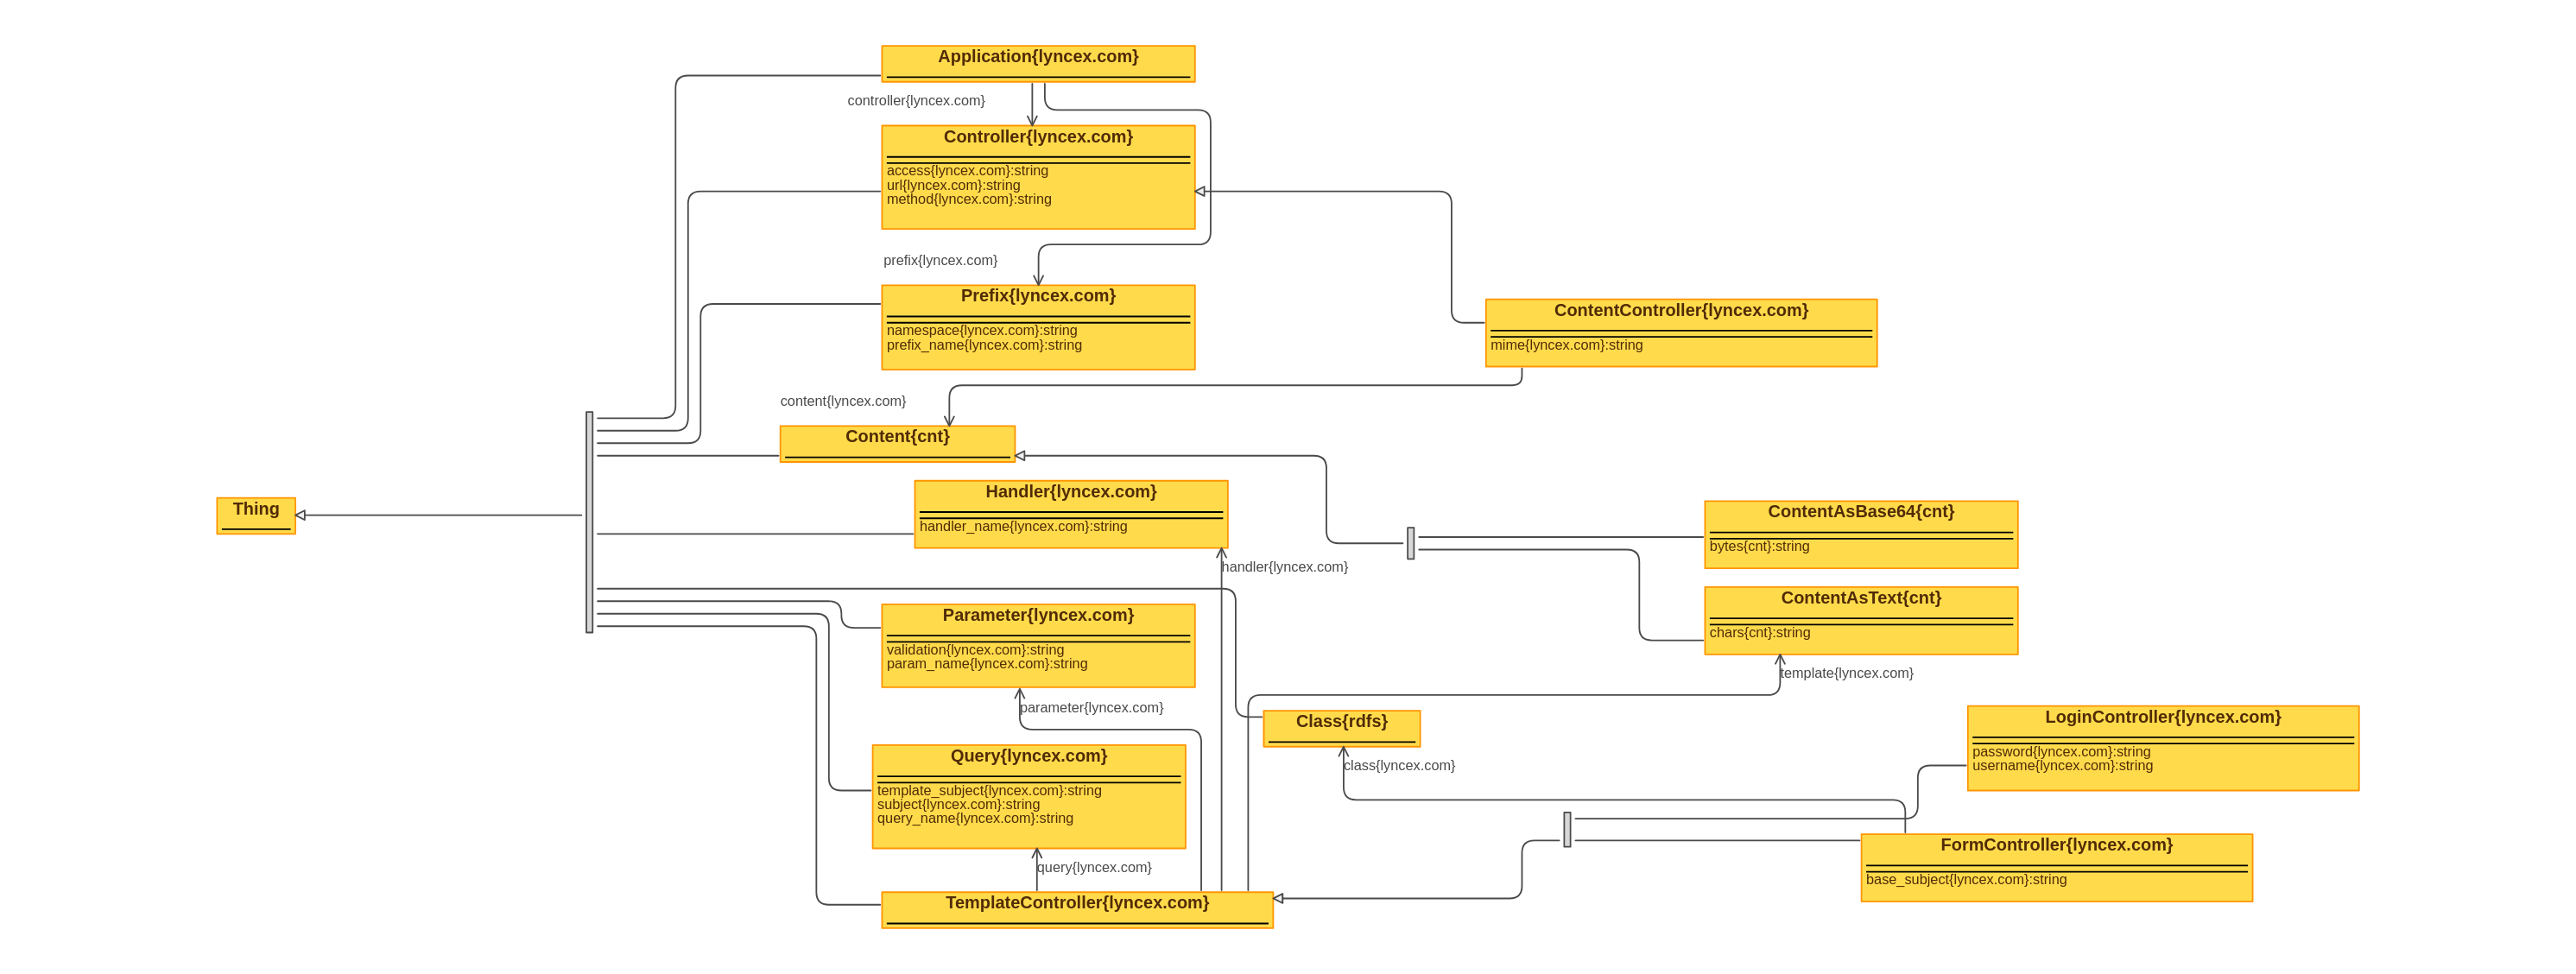
\includegraphics[width=\textwidth]{lyncex.png}
    \caption{Ontología de Lyncex}
    \label{fig:ontologia}
\end{figure}

\chapter{Componentes del sistema}
Lyncex es una aplicación Prolog que se ejecuta a modo de servidor. Se recomienda utilizar la aplicación desde un contenedor Docker, si bien no es estrictamente necesario. 
Una vez lanzado, la única forma de interactuar con el sistema es mediante la API.

\section{API}
La API de Lyncex se encarga de que el sistema interactúe con el exterior.
Un programador que desee crear una aplicación de Lyncex es lo único que debería tocar.
Externamente se trata de una API HTTP, que define varias rutas bajo la ruta \_api.
Las operaciones que soporta la API son:
\begin{itemize}
    \item Creación de tripletas en la base de datos (POST, \_api)
    \item Borrado de tripletas de la base de datos (DELETE, \_api/delete) con posibilidad de aplicar filtros
    \item Lectura de tripletas de la base de datos (GET, \_api/query) con posibilidad de aplicar filtros
\end{itemize}

La creación de tripletas toma como entrada un fichero de tipo Turtle, mismo formato que se encuentra a la salida de la lectura de tripletas.
De esta forma, se pueden realizar backups rápidos de la aplicación.

El componente API además dispone de una validación elemental de RDF Schema.
Esto se consigue si tanto los datos como las ontologías que los definen coexisten en la aplicación.
Se verifica básicamente el uso correcto de instancias y propiedades mediante rdfs:domain.
Técnicamente, RDF Schema no es un lenguaje de validación al uso, sino más bien de descripción de datos, pero demasiado abierto como para hacer comprobaciones estrictas.
Es por ello que solo se valida este único comportamiento.


\section{Controladores}
Los controladores son los componentes que implementan la funcionalidad principal definida por la ontología.
Al llegar una petición, se van probando los diferentes tipos de controladores hasta encontrar uno que sea del tipo al definido en la tripleta: (Controlador, rdf:type, lyncex:TipoControlador).
Inicialmente se han diseñado tres controladores.

\subsection{ContentController}
El más básico de todos, simplemente devuelve lo que tenga definido en la tripleta (Controlador, lyncex:content, Content) con el tipo MIME 
de la tripleta (Controlador, lyncex:mime, MimeType). El nodo Content es del tipo ContentAsText o ContentAsBase64, permitiendo ambos modos de representación del contenido.
Ambos tipos forman parte de la ontología de W3C llamada \textit{Representing Content in RDF 1.0}\cite{cnt}.
El tipo ContentAsText está pensado para formatos de tipo texto (HTML, CSS, JavaScript) mientras que ContentAsBase64 está pensado para formatos binarios (imágenes, sonidos, etc).
Hay que mencionar, que en ningún caso almacenar ficheros binarios codificados en base 64 es una opción óptima y esta opción se ofrece más como una conveniencia.

\begin{figure}[h]
    \centering
    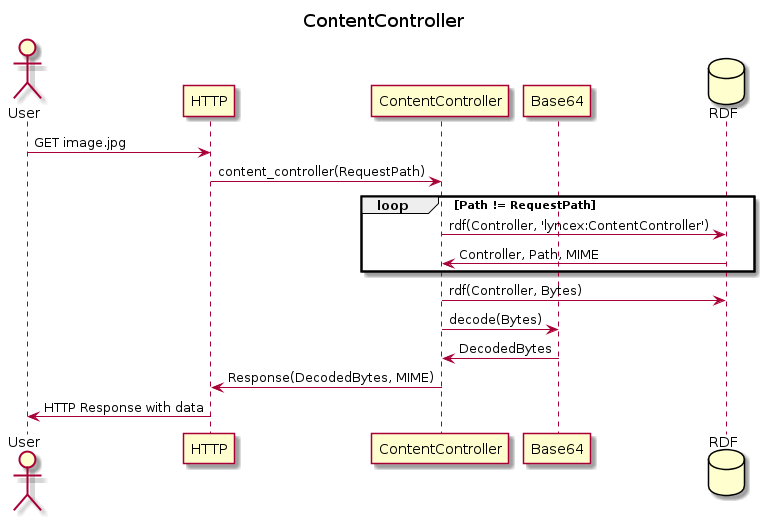
\includegraphics[width=\textwidth]{plantuml/contentcontroller.png}
    \caption{Diagrama de secuencia del ContentController}
    \label{fig:contentcontroller}
\end{figure}

\subsection{TemplateController}
El TemplateController se encarga de gestionar las plantillas. Estas plantillas se definen siguiendo la sintaxis Semblance de la librería simple-template.
El TemplateController realiza las siguientes operaciones en orden:
\begin{enumerate}
    \item Procesado de parámetros GET y POST definidos previamente por instancias lyncex:Parameter
    \item Templatizado de queries (si lo hubiera) especificadas (instancias de lyncex:Query)
    \item Resolución de las queries (si hubiera)
    \item Ejecución de los handlers (si hubiera) (instancias de lyncex:Handler)
    \item Templatizado final
\end{enumerate}

\begin{figure}[h]
    \centering
    \includegraphics[width=\textwidth]{plantuml/templatecontroller.png}
    \caption{Diagrama de secuencia del TemplateController}
    \label{fig:templatecontroller}
\end{figure}

\subsection{FormController}
El FormController es una abstracción por encima del TemplateController a nivel interno, pero de cara a la ontología no es una subclase.
Su funcionamiento depende de si se realiza una petición POST o GET. Ante una petición POST, el controlador procesará los parámetros.
Buscará la existencia de un parámetro llamado \_id en primer lugar, ya que definirá el sujeto sobre el que se van a almacenar tripletas.
A continuación recorrerá el resto de parámetros. El nombre de cada parámetro es la URL de la propiedad y el valor será el valor de la propiedad.
Actualmente no se soporta crear dos tripletas de la misma propiedad en el mismo procesado.

Si tenemos una operación GET, el controlador leerá la clase base y todas las propiedades que pueda extraer de la clase. Para ello es importante que la ontología de los datos esté cargada, si no, no será capaz de adivinar qué propiedades admite la clase.
Una vez tenga el listado de propiedades, generará un formulario HTML ajustando todos los valores de forma adecuada al formato de aceptación del POST.

\begin{figure}[h]
    \centering
    \includegraphics[width=\textwidth]{plantuml/formcontroller-get.png}
    \caption{Diagrama de secuencia del FormController ante un GET}
    \label{fig:formcontrollerget}
\end{figure}

\begin{figure}[h]
    \centering
    \includegraphics[width=\textwidth]{plantuml/formcontroller-post.png}
    \caption{Diagrama de secuencia del FormController ante un POST}
    \label{fig:formcontrollerpost}
\end{figure}

\section{Procesado de parámetros}
El procesado de parámetros es llamado por diferentes controladores para adaptar el formato de entrada HTTP GET y POST a un formato común (un diccionario Prolog).
Solo saldrán del procesado aquellos parámetros indicados de forma explícita, ignorando aquellos que no lo estén.
Durante el procesado se ejecutan las validaciones si las hubiera. Existen dos tipos de validaciones: Regex y Prolog.
Cualquier parámetro puede tener cero, una o ambas validaciones.

La validación regex, simplemente comprueba que el valor del parámetro cumpla con el patrón de una expresión regular estándar. Por debajo se implementa mediante la librería PCRE.

La validación Prolog es código Prolog que define un término validation(X). Dentro de este código se puede llamar a cualquier código Prolog.
La validación será exitosa si el término se puede evaluar a true, en caso contrario, se considerará que el parámetro está mal y fallará.

En el caso del FormController, las validaciones tienen que ubicarse en otro lugar. Ya que el FormController importa implícitamente todos los parámetros de una ontología, no se puede adjutar una validación de la misma forma.
La solución si usamos un FormController es extender la propia ontología.
Así, en un sujeto de tipo rdf:Property, podemos añadir lyncex:validation y lyncex:code\_validation, que funcionan como validación regex y validación Prolog, respectivamente.

\chapter{Implementación}

\section{Herramientas de desarrollo}
\subsection{SWI Prolog}
SWI Prolog\cite{prolog} es un entorno de programación Prolog, ampliamente usado gracias a su condición de software libre, su portabilidad y 
su estrategia de baterías incluidas, que hace que disponga de gran cantidad de librerías y módulos por defecto.
La comunidad de SWI Prolog es pequeña pero activa y a parte de la gran cantidad de librerías, existe un sistema de packs, que permiten instalar librerías de terceros.

Entre los módulos que tiene SWI Prolog y que es difícil encontrar en otras implementaciones, debemos destacar los módulos de web semántica y RDF y los de HTTP.
Sin estos módulos, la realización de Lyncex hubiese sido mucho más compleja y alargada en el tiempo.

\subsection{RDF, Turtle}
RDF, siglas de Resource Description Framework, es un modelo de datos para describir datos usando tripletas sujeto-predicado-objeto. 
Se trata de un estándar del W3C y dispone de una variedad de sintaxis. Se ha elegido Turtle como sintaxis predeterminada ya que es la que en nuestra opinión es la más simple y menos verbosa.
Otros formatos alternativos como RDF/XML o JSON-LD parten de formatos diseñados para ser usados de forma diferente, añadiendo complejidad y verbosidad en el camino.

\subsection{IDE}
Como IDE se ha utilizado Visual Studio Code\cite{vscode}, un editor propiedad de Microsoft, pero multiplataforma.
Es un IDE con el que ya había familaridad previa y no supone ningún esfuerzo usarlo para este proyecto.
Visual Studio Code dispone de un sistema de plugins, y entre otros, hay plugins de Prolog y de Turtle.
El último fue usado para obtener resaltado de sintaxis, mientras que el primero se evaluó y finalmente se deshechó.
El motivo es que el plugin ejecuta Prolog por debajo para detectar errores de sintaxis, pero al tratarse de una aplicación que es un servidor, al ejecutarse toma los puertos y no podemos usarlos
en pruebas lanzadas a través de la terminal.

\subsection{Sistema operativo}
La totalidad del proyecto se ha realizado sobre Debian, en su versión Sid. Se trata de un sistema operativo con kernel Linux, 
de amplio uso en servidores, y también usado, en menor medida, en portátiles y workstations.

\subsection{Docker}
Para que los entornos de prueba y de ejecución sean reproducibles, se ha optado por usar Docker y su utilidad, Docker Compose.
Docker es un sistema de contenedores para Linux que proporciona capacidades de aislamiento y reproducibilidad de entornos similares a las máquinas virtuales, sin el overhead que usar estas conlleva.
Existen otros sistemas parecidos, como LXD, pero Docker tiene varias ventajas: poder describir entornos como código versionable (Dockerfile) y poder orquestar de forma sencilla entornos pequeños y medianos (docker-compose).

\subsection{Git y GitHub}
Para versionar el código fuente se ha usado el sistema Git, usando como almacenamiento GitHub. Principalmente se ha usado a través de la línea de comandos.
No se han aprovechado muchas de sus características de ramas y merges, ya que al ser un proyecto personal, solo se iba modificando una parte del programa a la vez.
Adicionalmente se ha hecho uso de la integración continua gratuita ofrecida por GitHub llamada GitHub Actions. De este modo se ha definido una acción que se ejecuta al recibir nuevo código en el repositorio.
Esta acción construía las imágenes de Docker necesarias y pasaba los tests de Behave y de PlUnit.

\subsection{Behave}
Para asegurarnos que las historias de usuario se implementaban correctamente se ha decidido usar Behave.
Se trata de un framework para definir tests en lenguaje Gherkin, un lenguaje muy similar al lenguaje natural. Estos tests se componen de pasos,
los cuáles son implementados en Python. Como las historias de usuario nos hablan de como debe reaccionar el sistema con el exterior, no hay problema en implementar los tests de este tipo en otro lenguaje.


\chapter{Validación y pruebas}

\section{Pruebas manuales}

\section{Tests unitarios}

\section{Test E2E}

\chapter{Aplicación de ejemplo}

\chapter{Manuales}

\section{Manual de instalación}

\section{Manual de usuario}

\chapter{Conclusiones y trabajo futuro}

\begin{appendices}
\chapter{Ontología}
\lstinputlisting{lyncex.ttl}
\end{appendices}
\bibliographystyle{acm}

\bibliography{ref}

\end{document}


% Los objetivos principales que se propusieron para Lyncex y que debían ser cumplidas son:

% \begin{itemize}
%     \item US1: Almacenar tripletas de datos junto a sus ontologías en el mismo espacio, validándose
%     \item US2: Desarrollar una ontología que permita definir aplicaciones web sobre datos almacenados en el propio almacenamiento
%     \item US3: Servir páginas web estáticas
%     \item US4: Servir páginas web que necesiten leer datos del almacenamiento (plantillas)
%     \item US5: Servir páginas web con formularios
% \end{itemize}

% Otros objetivos que estaría bien cumplir, pero no son necesarios para tener una versión funcional son:
% \begin{itemize}
%     \item OUS1: Servir páginas web con sistemas de autenticación y autorización propios
%     \item OUS2: Servir APIs web de forma similar al contenido HTML
%     \item OUS3: Tener un endpoint de consulta SPARQL
% \end{itemize}